\documentclass[../CSC_52081_EP.tex]{subfiles}

\begin{document}
\section{Methodology / Approach}


\subsection{Environment and Agent Implementation}
\label{sec:CNN}

This study employs the CarRacing-v3 environment from Gymnasium \cite{gymnasium}, a challenging benchmark characterized by high-dimensional visual observations and multiple action modalities. In order to transform the observation space (a 3x96x96 picture frame) in the action space supported by the environment, we implemented a Convolutional Neural Network (CNN) inspired by \cite{DQN_CNN} with the following characteristics:

\begin{itemize}
    \item \textbf{Image}: the frames are transformed from an RGB state representation to grayscale, and the resolution is downscaled to 84x84 pixels. These steps facilitate the network computations, making them less complex. Additionally, to allow the network to accurately track the car's dynamics and improve the agent's ability to adjust actions based on the current state, each frame is stacked with the previous three frames. As a result, every state is represented by a sequence of four consecutive grayscale frames at 84x84 resolution (see Figure \ref{fig:grayscale}).

    \item \textbf{Input Layer}: 4-channel 84x84 images.
    
    \item \textbf{First Convolutional Layer}: 16 filters, 8x8 kernel, stride 4, ReLU activation. After applying the convolution, the output have dimensions 20x20.

    \item \textbf{Second Convolutional Layer}: 32 filters, 4x4 kernel, stride 2, ReLU activation. After applying the convolution, the output have dimensions 9x9.

    \item \textbf{Flatten Layer}: The output from the second convolutional layer is flattened into a 1D vector. The size of this vector is 32 * 9 * 9 = 2592.

    \item \textbf{First Fully Connected (FC) Layer}: 256 neurons, ReLU activation.

    \item \textbf{Second Fully Connected (FC) Layer}: The last fully connected layer defines the action space of the environment. For discrete action-space trials (DQN and Deep SARSA), this layer consists of five neurons with a linear activation function. In contrast, for continuous action-space tests (PPO, SAC, and CEM), the output layer comprises three neurons with different activation functions: \textit{tanh} for the steering action (ranging from [-1, 1]) and \textit{sigmoid} for the gas and brake actions (both ranging from [0, 1]).
\end{itemize}

\begin{figure}[H]
    \centering
    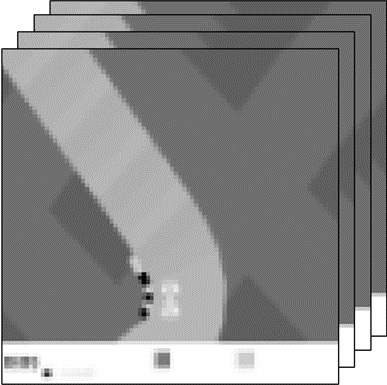
\includegraphics[scale = 0.3]{figures/grayscale_4.png}
    \caption{Input observation space for the CNN, composed by four grayscale consecutive frames from the car racing environment. Reference: \cite{DQN_CNN}}
    \label{fig:grayscale}
\end{figure}

\begin{figure}[H]
    \centering
    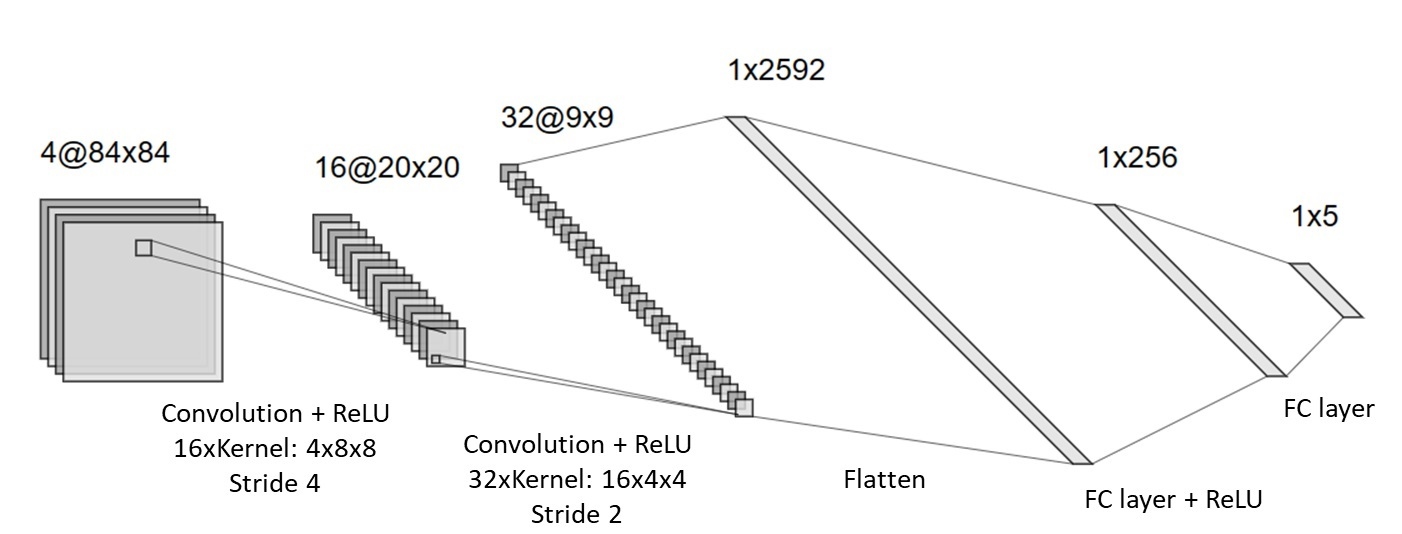
\includegraphics[scale = 0.15]{figures/CNN.png}
    \caption{Convolutional Neural Network (CNN) architecture for processing the observation from the car racing environment. Reference: \cite{DQN_CNN}}
    \label{fig:CNN}
\end{figure}

\subsection{Replay Buffer}
A key innovation introduced in the original DQN paper is the concept of experience replay. This technique involves storing experiences in a replay memory buffer, allowing the agent to break the temporal dependencies between consecutive experiences. During training, random minibatches are sampled from this buffer, which improves the stability of the learning process.

\subsection{Algorithms Design}

\hspace{1cm}

\subsubsection{DEEP Q-Network (DQN)}
The model is trained by optimizing a loss function based on the temporal difference error between predicted and target Q-values. 

For the DQN, the target network consists in maintaining two separate networks: the main (or online) network, which is used for learning and selecting actions, and the target network, which is updated less frequently. The target network is a copy of the online network, and its parameters are periodically updated by copying the parameters of the online network to it. This approach helps stabilize the learning process by providing a fixed target for the updates, preventing oscillations and divergence in the Q-value estimates.

Training is conducted on minibatches of state-action-reward-next state sequences sampled from the replay buffer. The update rule of the algorithm is given by:
    \begin{equation}
        Q(s, a) \leftarrow Q(s, a) + \alpha \left[ r + \gamma \max_{a'} Q(s', a') - Q(s, a) \right]
    \end{equation}
    
    where $\max_{a'} Q(s', a')$ is the maximum Q-value at the next state $s'$ (greedy selection).

\hspace{1cm}

\subsubsection{DEEP SARSA}
For the SARSA algorithm, learning is performed using a single Q-network instead of maintaining a separate target network. The algorithm follows an on-policy approach, where the agent updates its Q-values based on the actions it actually takes, rather than using a target derived from the maximum possible future reward. This ensures that updates remain consistent with the agent’s current policy.

Training is conducted on minibatches of state-action-reward-next state-next action sequences sampled from the replay buffer. The update rule of the algorithm is given by:

\begin{equation}
        Q(s, a) \leftarrow Q(s, a) + \alpha \left[ r + \gamma Q(s', \pi(s')) - Q(s, a) \right]
    \end{equation}

where $Q(s', \pi(s'))$ corresponds to the Q-value of the next state-action pair, following the agent’s current policy ($\epsilon$-greedy). This approach ensures that the learning process accounts for the agent’s actual behavior, rather than assuming a greedy action selection at every step.

\hspace{1cm}

\subsubsection{Proximal Policy Optimization (PPO)}
The training for the PPO is described as follows:

\begin{itemize}
    \item First, we collect trajectories from the environment:
    \[
    \mathcal{D} = \{ (s_t, a_t, r_t, s_{t+1}) \}_{t=0}^{T}
    \]
    where:
    \( s_t \) is the state at time \( t \), \( a_t \) is the action taken, \( r_t \) is the reward received, and \( s_{t+1} \) is the next state.

    \item Compute Advantage Estimates Using GAE. The temporal difference (TD) residual is given by:
    \[
    \delta_t = r_t + \gamma V(s_{t+1}) - V(s_t)
    \]
    
    The Generalized Advantage Estimation (GAE) is computed recursively:
    
    \[
    A_t^{GAE} = \delta_t + (\gamma \lambda) A_{t+1}^{GAE}
    \]
    
    where \( \gamma \) is the discount factor and \( \lambda \) is the GAE smoothing parameter.

    The estimated return is:

    \[
    \hat{R}_t = A_t^{GAE} + V(s_t)
    \]

    \item Compute the Probability Ratio:

    \[
    r_t(\theta) = \frac{\pi_{\theta}(a_t | s_t)}{\pi_{\theta_{\text{old}}}(a_t | s_t)}
    \]
    
    where \( \pi_{\theta} \) is the current policy, and \( \pi_{\theta_{\text{old}}} \) is the old policy before the update.

    \item Clipped Surrogate Objective, to prevent large policy updates:

    \[
    L^{\text{CLIP}}(\theta) = \mathbb{E} \left[ \min \left( r_t(\theta) A_t, \text{clip}(r_t(\theta), 1 - \epsilon, 1 + \epsilon) A_t \right) \right]
    \]
    
    where \( \epsilon \) is a small clipping parameter (\( 0.2 \) in our code).

    \item Compute Value Function Loss:

    \[
    L^{\text{VF}}(\theta) = \mathbb{E} \left[ (V_{\theta}(s_t) - \hat{R}_t)^2 \right]
    \]

    \item To encourage exploration, an entropy bonus is added:

    \[
    L^{\text{ENTROPY}}(\theta) = \mathbb{E} \left[ -\pi_{\theta}(a_t | s_t) \log \pi_{\theta}(a_t | s_t) \right]
    \]

    \item The total loss function combines policy loss, value loss, and entropy:
    
    \[
    L(\theta) = L^{\text{CLIP}}(\theta) - c_1 L^{\text{VF}}(\theta) + c_2 L^{\text{ENTROPY}}(\theta)
    \]
    
    where \( c_1 \) and \( c_2 \) are coefficients.
    
    \item The policy parameters are updated via gradient ascent:
    
    \[
    \theta \leftarrow \theta + \alpha \nabla_{\theta} L(\theta)
    \]
    
    where \( \alpha \) is the learning rate.
    
\end{itemize}

Unlike other algorithms, we used two Neural Networks (NNs): one for the policy and another for the value function. The Policy Network follows the CNN architecture described in Section \ref{sec:CNN}, with its output representing the mean and standard deviation of the action distribution. Within the PPO class, the update function constructs a normal distribution based on these parameters, from which an action is sampled. The action is then clipped to ensure it stays within the boundaries of the continuous action space.

The Value Network, in contrast, uses a simplified version of the CNN, as it does not require extensive feature extraction. Its output is a single scalar representing the estimated state value.

\hspace{1cm}
\subsubsection{CEM}


\hspace{1cm}
\subsubsection{SAC}



\subsection{Comparison and Evaluation Methods}

\subsubsection{Action-Space Design}
We compare the efficiency of discrete versus continuous action spaces by analyzing convergence rates, stability, and final policy performance across different action representations.

\subsubsection{Hyperparameter Sensitivity Analysis}
We investigate the stability and convergence dynamics under different step-size configurations by adapting the learning rate.

\subsubsection{Performance Metrics}
Our evaluation framework incorporates several key indicators to comprehensively assess the performance of the implemented methodologies. Firstly, cumulative rewards are used to quantify the overall policy efficiency and long-term reward accumulation. Secondly, convergence speed is measured by the number of training episodes required to reach a stable performance threshold. Thirdly, sample efficiency is evaluated by assessing the learning progress per unit of environmental interaction, which helps determine the algorithmic effectiveness. Lastly, robustness evaluation is conducted through perturbation tests under varying environmental conditions to gauge the model's adaptability and resilience.


\subsection{Visual Analysis and Interpretation}
To further refine our understanding of agent behavior and policy effectiveness, we employ several visualization techniques:

\subsubsection{Learning Curves}
We analyze episodic reward trends over the course of training to identify key inflection points and phases in the learning process. This involves plotting the cumulative rewards obtained in each episode, which helps in diagnosing the learning stability, convergence behavior, and potential over-fitting or under-fitting issues. By examining these curves, we can infer the efficiency of the learning algorithm and the impact of different hyperparameter settings.


\subsubsection{Final Policy Comparisons}
We conduct a comparative analysis of the final policies learned under different training configurations. This involves contrasting the strategies and behaviors exhibited by the agent after the training process is complete. In order to compare algorithm performance under the same conditions of an environment (which is randomly generated), we fixed a seed variable upon its generation to maintain the main caracteristics.

By systematically comparing these policies, we can infer the impact of various algorithmic choices, such as different exploration strategies, reward structures, or network architectures, on the overall performance and robustness of the learned policies. This comparative analysis provides a deeper understanding of the strengths and limitations of each approach, guiding future improvements and refinements.


\subsection{Reproducibility}
All implementations utilie OpenAI Gymnasium, PyTorch/TensorFlow for training, and Stable-Baselines3 for baseline comparisons. The full codebase is available at \href{https://github.com/tr0fin0/ensta_CSC_52081_EP_project}{GitHub} to facilitate reproducibility.



\end{document}
